\documentclass[a4paper, 12pt, final, garamond]{book}
\usepackage{cours-preambule}

\raggedbottom

\makeatletter
\renewcommand{\@chapapp}{Travaux pratiques -- TP}
\makeatother

\let\SavedIndent\indent
\protected\def\indent{%
  \begingroup
    \parindent=\the\parindent
    \SavedIndent
  \endgroup
}
\setlength{\parindent}{0pt}

\begin{document}
\setcounter{chapter}{2}

\chapter{Formation et observation d'images \`a l'infini~: utilisation de la
lunette autocollimatrice}

\section{Objectifs}

\begin{itemize}
    \item Utiliser une lunette autocollimatrice pour~:
        \begin{enumerate}
            \item Reconnaître un faisceau parallèle~;
            \item Utiliser un faisceau parallèle~;
        \end{enumerate}
    \item Continuer à se familiariser avec un viseur à frontale fixe. 
    \item Utiliser la calculatrice pour réaliser des régressions linéaires.
\end{itemize}

\section{S'approprier}

\subsection{Principe de la lunette autocollimatrice}

\begin{wrapfigure}[9]{r}{0.6\textwidth} 
    \vspace{-60pt}
    \begin{center}
        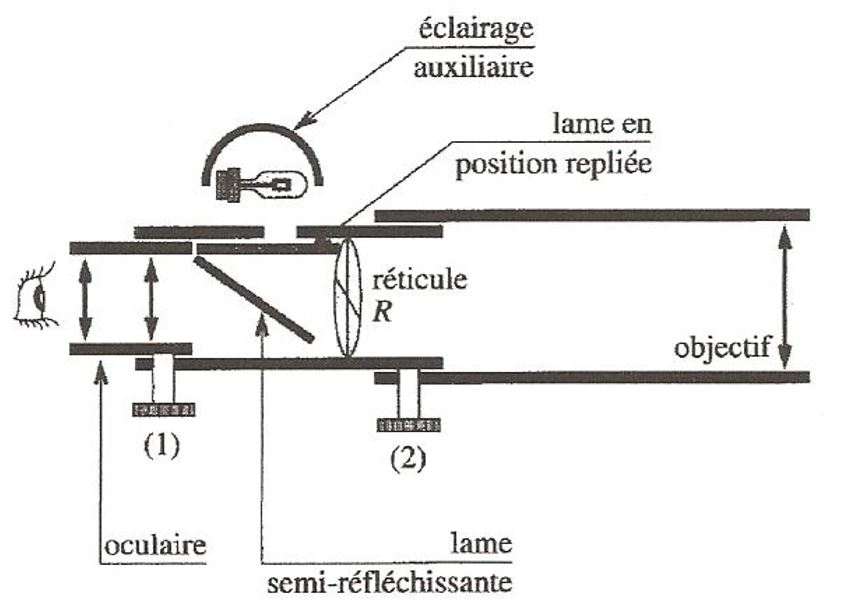
\includegraphics[width=0.55\textwidth]{lunette_auto}
    \end{center}
    \vspace{-80pt}
\end{wrapfigure} 

La lunette autocollimatrice permet de réaliser un faisceau de lumière parallèle.
Elle est constituée d'un objectif, d'un réticule $R$ et d'un oculaire. Entre
l'oculaire et le réticule est disposée une lame semi-réfléchissante, inclinée à
$45°$ par rapport à l'axe optique du dispositif et éclairée par une petite
ampoule (éclairage auxiliaire).

\vspace{2cm}

\subsection{Théorème des vergences}

Considérons deux lentilles minces $\mathcal{L}_1$ et $\mathcal{L}_2$ de centres
optiques respectifs $O_1$ et $O_2$ et de distances focales images respectives
$f'_1$ et $f'_2$. On suppose que ces deux lentilles sont accolées si bien que
leurs centres optiques sont confondus~: $O_1 \equiv O_2 \equiv O$. Soit un objet
$AB$ conjugué à son image $A_2B_2$ par le doublet de lentilles. Par ailleurs, on
introduit $A_1B_1$ l'image intermédiaire. Nous pouvons alors écrire la relation
de conjugaison de Descartes pour chacune des lentilles~: 

\centers{$\DS\frac{1}{\overline{OA_1}}-\frac{1}{\overline{OA}} = \frac{1}{f'_1}
    \qquad\text{et}\qquad \frac{1}{\overline{OA_2}}-\frac{1}{\overline{OA_1}} =
\frac{1}{f'_2}$} 

Sommons terme à terme ces deux relations. Il vient alors~: 

\centers{$\DS\frac{1}{\overline{OA_2}}-\frac{1}{\overline{OA}} =
\frac{1}{f'_1}+\frac{1}{f'_2}$}

Si bien que tout se passe comme si le système optique était équivalent à une
unique lentille mince de distance focale image $f'_{\rm eq}$ tel que~: 

\centers{$\DS\frac{1}{f'_{\rm eq}}= \frac{1}{f'_1}+\frac{1}{f'_2}$}

\leftencadre{Soit encore, en terme de vergences~: }{$V_{\rm eq} = V_1+V_2$}

\underline{Remarque}~: Même si cette relation n'est pas explicitement au
programme, il est bon de connaître cette propriété. 

\section{Réaliser~: réglage de la lunette autocollimatrice}

\subsection{Réglage de l'oculaire}

Même principe que pour régler le viseur~:

\begin{enumerate}
    \item Allumer la lampe latérale de la lunette qui éclaire le réticule.
        \textbf{Attention} elle doit être alimentée en $\SI{6}{V}$ alternatif.
        Sinon vous risquez de l'endommager.
    \item Régler l'oculaire à votre vue~: mettre au point le réticule en
        agissant sur l'œilleton de l'oculaire grâce à la vis (1). Ce réglage est
        personnel et nécessaire avant toute manipulation~; La lunette est réglée
        quand on voit les deux fils croisés nets.
\end{enumerate}

\subsection{Réglage de la lunette sur l'infini}

On effectue ce réglage pour obtenir un faisceau de lumière parallèle. Il se fait
à l'aide d'un miroir plan. 

\bigskip

Démarche à suivre~:
\begin{enumerate}
    \item Placer la lame semi-réfléchissante interne de telle façon que la
        lumière sorte de l'objectif (loquet argenté). Pour cela, vérifier qu'un
        faisceau lumineux est visible en mettant votre main à la sortie de la
        lunette.
    \item Placer sur l'objectif (immédiatement après la lunette) le petit miroir
        plan.
    \item Observer l'image en retour du réticule: déplacer l'ensemble oculaire
        par rapport à l'objectif de façon à ce que cette image en retour soit
        aussi nette que l'objet, en agissant sur la bague moletée (2) de la
        lunette.
\end{enumerate}

\bigskip

On vient alors de réaliser un réglage par autocollimation. Ainsi, on s'assure
que le réticule est au foyer objet de l'objectif. 

\bigskip

La lunette peut ainsi être utilisée~:
\begin{itemize}
    \item Pour reconnaître un faisceau parallèle (1er montage),
    \item Comme source de faisceau parallèle (2ème montage).
\end{itemize}

\section{Valider}

\subsection{Détermination d'une distance focale}

L'objectif de cette partie est de déterminer la distance focale d'une lentille
expérimentalement (focométrie) par reconnaissance d'une faisceau parallèle en
utilisant la lunette autocollimatrice. 

\subsubsection{Montage}

  \begin{center}
    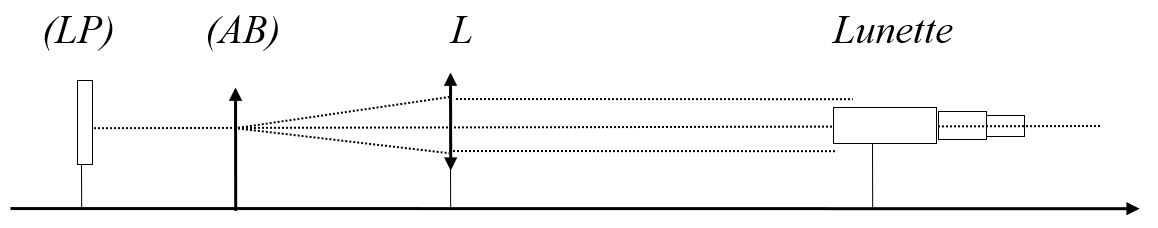
\includegraphics[width=0.8\textwidth]{1}
  \end{center}
  
\begin{enumerate}
    \item  Prendre comme objet $AB$, la plaque constituée des lettres $F$ sur
        support translucide et prendre une lentille de distance focale
        $\SI{10}{cm}$ ou $\SI{20}{cm}$. Éclairer l'objet $AB$ avec la lampe
        spectrale $(LP)$. Cette lampe doit être allumée une dizaine de minutes
        avant l'expérience pour chauffer. Interposer un dépoli devant la lampe
        pour limiter la luminosité et protéger vos yeux. 
    \item  Réaliser le montage ci-dessus, en mettant la lunette à droite de la
        lentille, sa place a peu d'importance. La lame semi-réflechissante à
        l'intérieur de la lunette doit être rétractée.
    \item  Déplacer la lentille pour voir dans la lunette autocollimatrice
        l'image $A'B'$ de $AB$  nette sur le réticule~: $A'B'$ est alors à
        l'infini donc $AB$ est dans le plan focal objet de la lentille. 
\end{enumerate} 

\subsubsection{Mesure de la distance focale}

On peut alors estimer la distance focale $f'$ de la lentille en mesurant grâce
au réglet fixé sur le banc optique la distance entre l'objet et la lentille. Si
vous constatez un désaccord trop grand entre la valeur prévue et la valeur
obtenue, essayez de trouver la cause de l'erreur systématique qui est créée par
le montage. Ce montage est moins précis que celui vu au TP précédent pour
déterminer la distance focale d'une lentille, mais il est également bien plus
rapide !

\bigskip

Vérifier que la position de la lunette n'a pas d'importance en la déplaçant sur
le banc optique, ce qui montre l'existence d'un faisceau de lumière parallèle.

\subsection{Vérification du théorème des vergences}

\subsubsection{Montage}

\begin{center}
    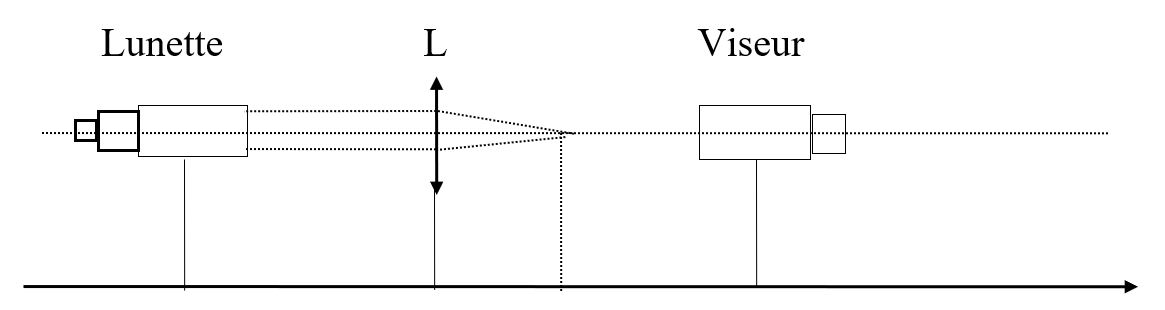
\includegraphics[width=0.8\textwidth]{2}
\end{center}
  
\begin{enumerate}
    \item Éteindre la lanterne utilisée dans le montage précédent. La source
        secondaire de la lunette autocollimatrice est maintenant la source de
        lumière~; La mettre à gauche sur le banc d'optique. Elle doit toujours
        être réglée sur l'infini. Interposer une lentille convergente entre la
        lunette et un viseur à frontale fixe. Soignez vos alignements.

    \item Repérer la position du viseur à frontale fixe permettant d'observer
        la face de sortie de la lentille (mettre un petit morceau de papier sur
        cette face ou la mine de votre crayon). On notera cette position $x_0$.

    \item Ensuite, viser l'image du réticule avec le viseur et relever la
        position $x_{R}$ du viseur à frontale fixe correspondante sur le banc
        optique. Vous chercherez cette position en éloignant le viseur d'environ
        la distance focale de la lentille par rapport à la position $x_0$
        précédemment obtenue. 

    \item En déduire la distance focale $f'$ de la lentille.

    \item Refaire la manipulation avec les différentes lentilles convergentes
        dont vous disposez. Vous ordonnerez vos résultats dans un tableau où
        vous préciserez pour chaque lentille la distance focale $f'$
        constructeur (celle inscrite sur les montures) et expérimentale
        (celle que vous venez de mesurer).   
\end{enumerate}
  
\subsubsection{Validation du théorème des vergences}
  
\begin{enumerate}

    \item  Prendre la lentille convergente de distance focale connue $+8\delta$. 
    
    \item  Associer à cette lentille (en les disposant accolées à la première),
        une par une, les autres lentilles dont vous disposez (convergentes ou
        divergentes). 
    
    \item  En utilisant la méthode précédente, mesurer la distance focale totale
        $f'_{\rm tot}$ pour chaque association de lentilles, et en déduire la
        vergence expérimentale de l'ensemble.
    
    \item  Réaliser au moins cinq associations différentes. Pour chacune des
        associations réalisées, vous compléterez un tableau contenant les
        colonnes suivantes~: vergence de la lentille ajoutée / vergence totale
        théorique du doublet / $x_0$ / distance focale expérimentale / vergence
        totale expérimentale. La distance $x_0$ est considéré comme étant la
        position du viseur lorsque l'on vise le centre optique des deux
        lentilles accolées. Il est mesuré comme la valeur moyenne des positions
        des faces externes des deux lentilles accolées. 
    
    \item  Réaliser ensuite une régression linéaire à la calculatrice de la
        vergence totale expérimentale en fonction de la vergence ajoutée pour
        chacune des lentilles. 
    
    \item  Relever les valeurs de $a$ (coefficient directeur), $b$ (ordonnée à
        l'origine) et $r$ (coefficient de corrélation) données par la
        calculatrice.
    
    \item  Ces valeurs de $a$ et $b$ vous semblent-elles cohérentes ? La valeur
        de $r$ traduit-elle un bon modèle ?
\end{enumerate}

\end{document}
